\clearpage
\paragraph{Soggetto 2}~

Di seguito vengono presentate alcune alcune misurazioni effettuate su un soggetto di sesso femminile, di età 41 anni e carnagione chiara. Il soggetto si trovava in condizioni di riposo.

\paragraph{MAX86916}~

Di seguito sono riportati i risultati ottenuti utilizzando il sensore MAX86916.

\subparagraph{Polpastrello indice sinistro}


\begin{figure}[h]
	\centering
	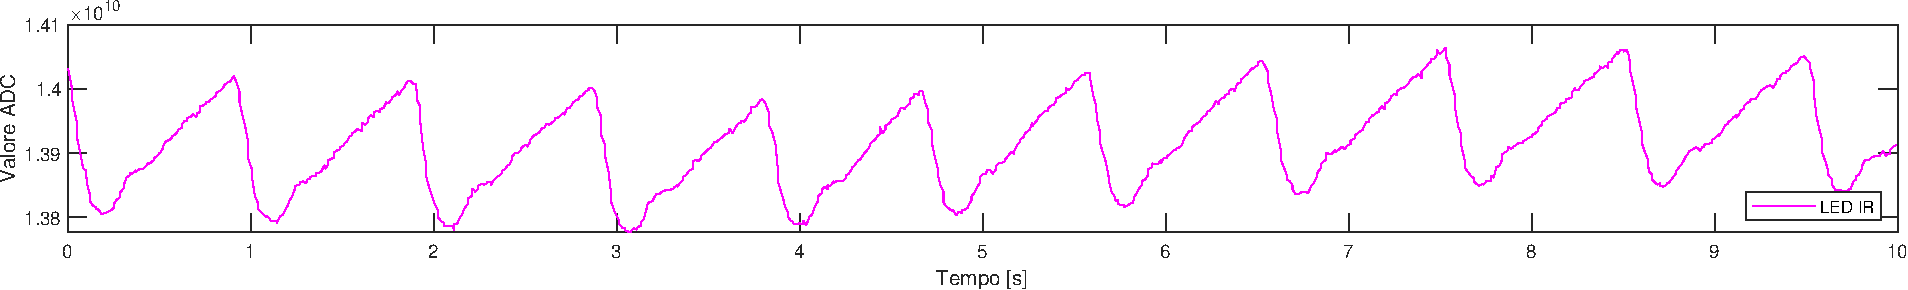
\includegraphics[width=1\linewidth]{ImageFiles/Misure Preliminari/Soggetto 2/max86916/polpastrello_ired}
	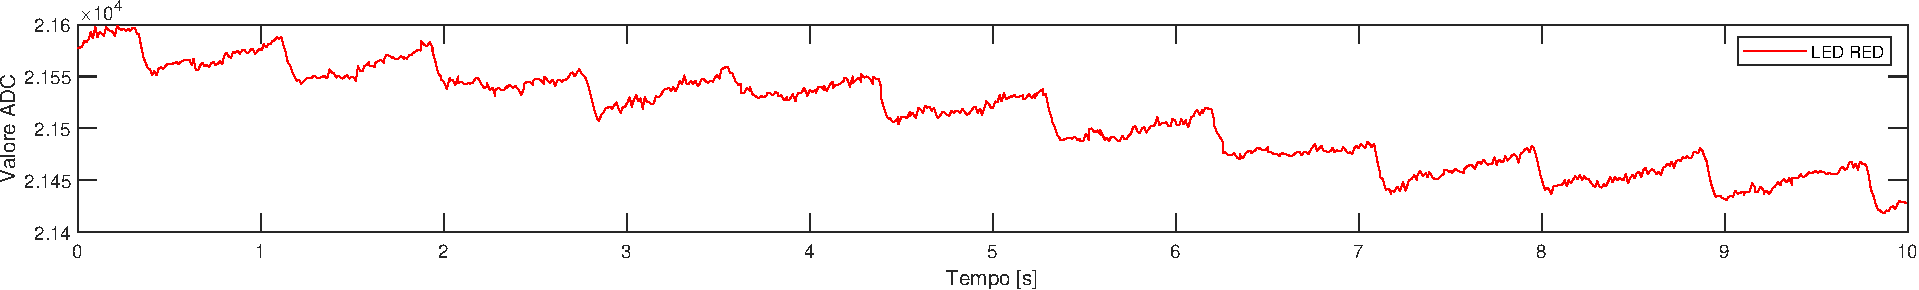
\includegraphics[width=1\linewidth]{ImageFiles/Misure Preliminari/Soggetto 2/max86916/polpastrello_red}
	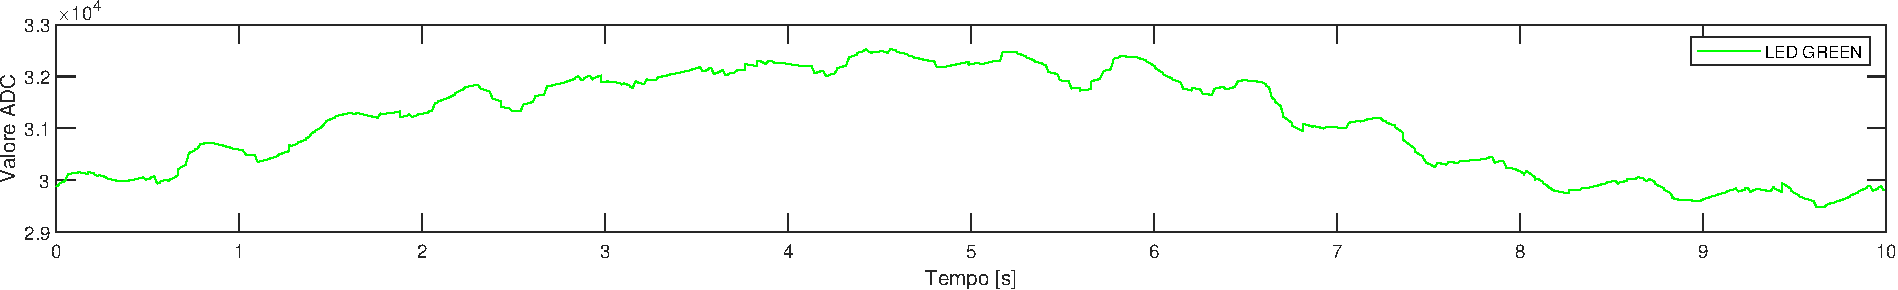
\includegraphics[width=1\linewidth]{ImageFiles/Misure Preliminari/Soggetto 2/max86916/polpastrello_green}
	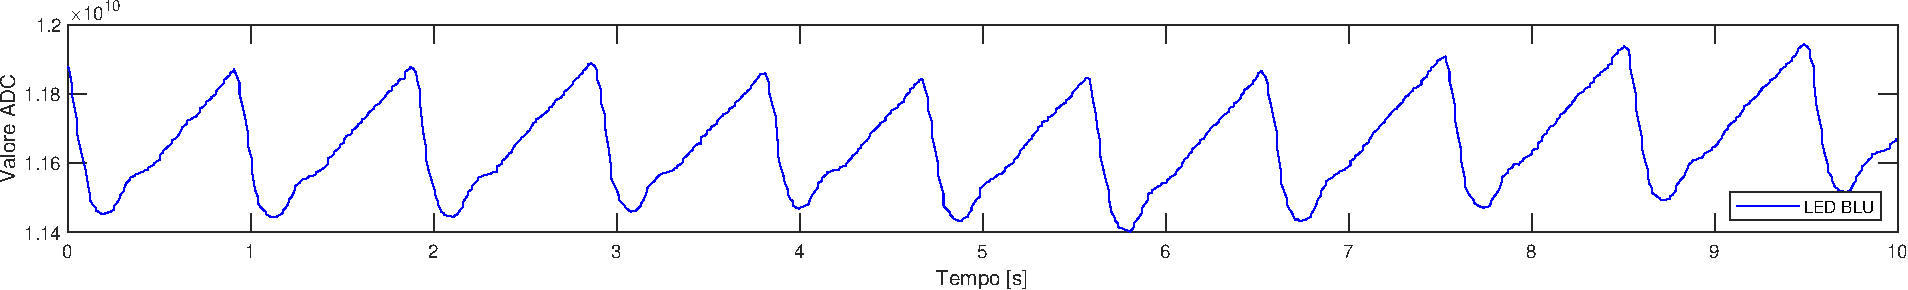
\includegraphics[width=1\linewidth]{ImageFiles/Misure Preliminari/Soggetto 2/max86916/polpastrello_blu}
	\caption{Segnali PPG acquisiti sul polpastrello del dito indice sinistro.}
	\label{fig:soggetto2_MAX86916_polpastrello}
\end{figure}

\clearpage

\subparagraph{Lobo orecchio destro}


\begin{figure}[h]
	\centering
	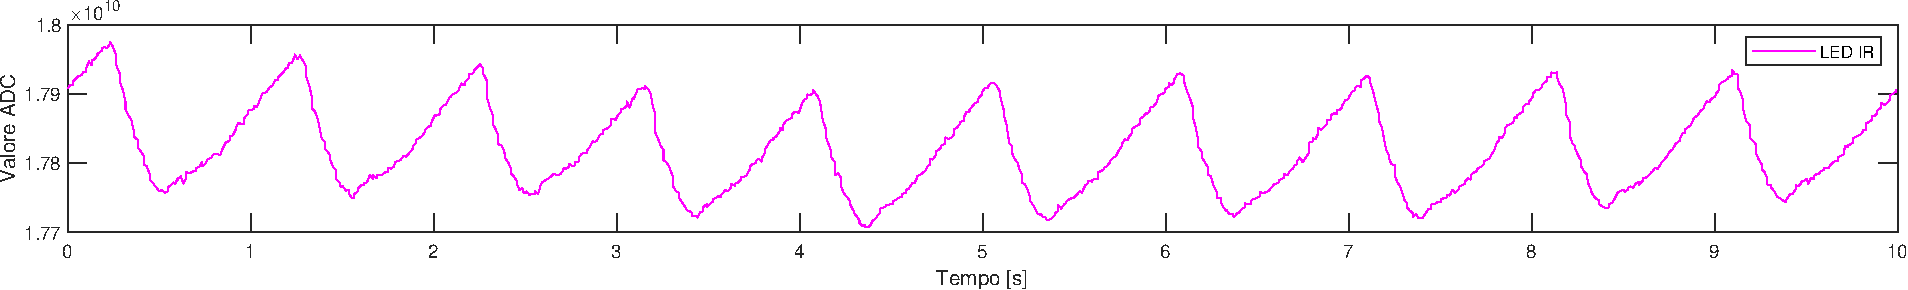
\includegraphics[width=1\linewidth]{ImageFiles/Misure Preliminari/Soggetto 2/max86916/lobo_ired}
	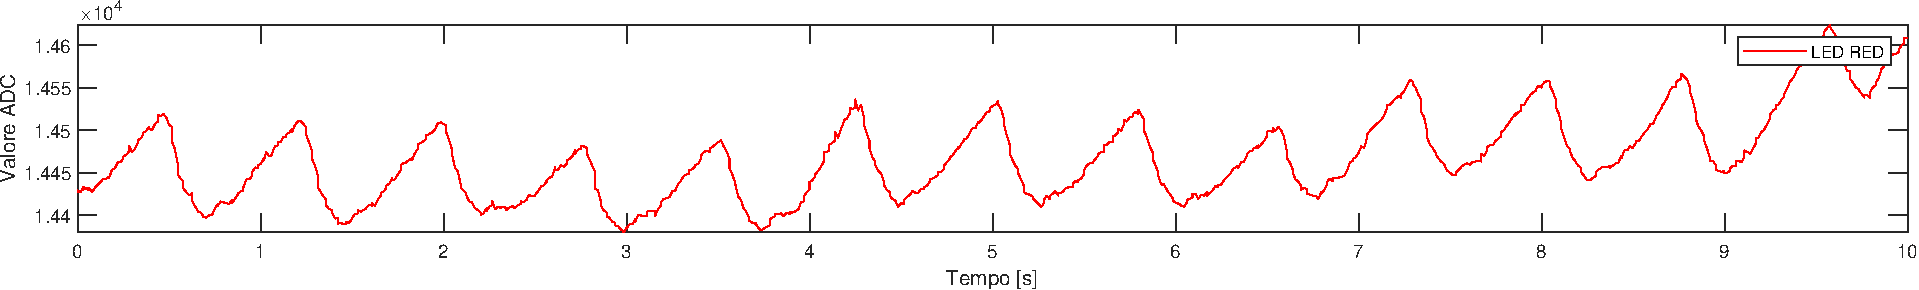
\includegraphics[width=1\linewidth]{ImageFiles/Misure Preliminari/Soggetto 2/max86916/lobo_red}
	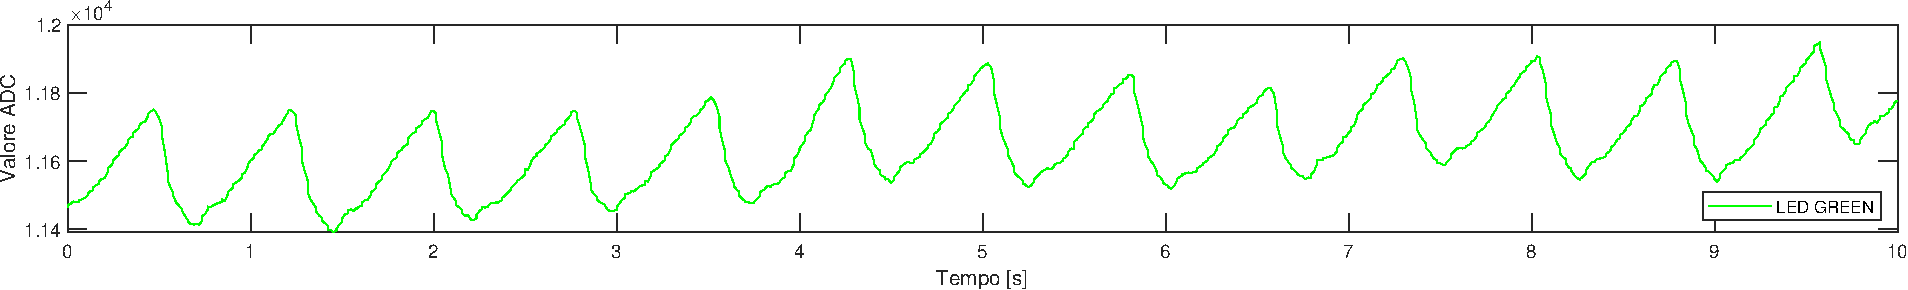
\includegraphics[width=1\linewidth]{ImageFiles/Misure Preliminari/Soggetto 2/max86916/lobo_green}
	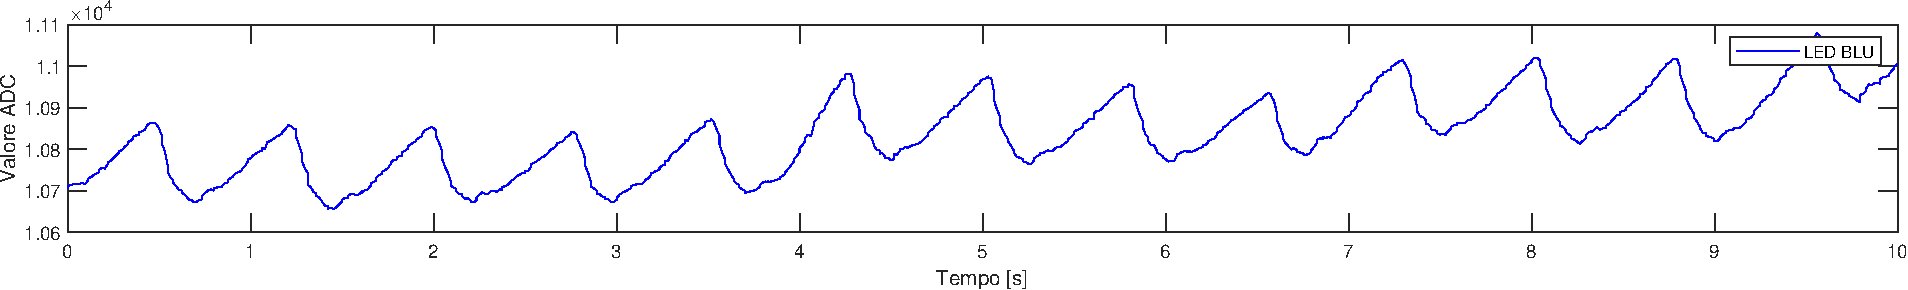
\includegraphics[width=1\linewidth]{ImageFiles/Misure Preliminari/Soggetto 2/max86916/lobo_blu}
	\caption{Segnali PPG acquisiti sul lobo dell'orecchio destro.}
	\label{fig:soggetto2_MAX86916_lobo}
\end{figure}

\subparagraph{Polso antero-interno}


\begin{figure}[h]
	\centering
	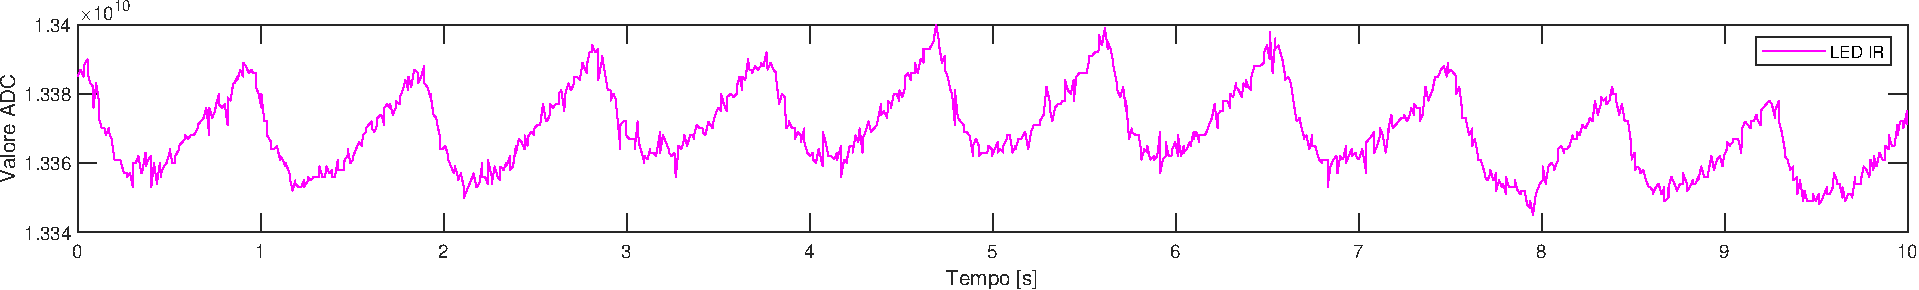
\includegraphics[width=1\linewidth]{ImageFiles/Misure Preliminari/Soggetto 2/max86916/polso_inferiore_ired}
	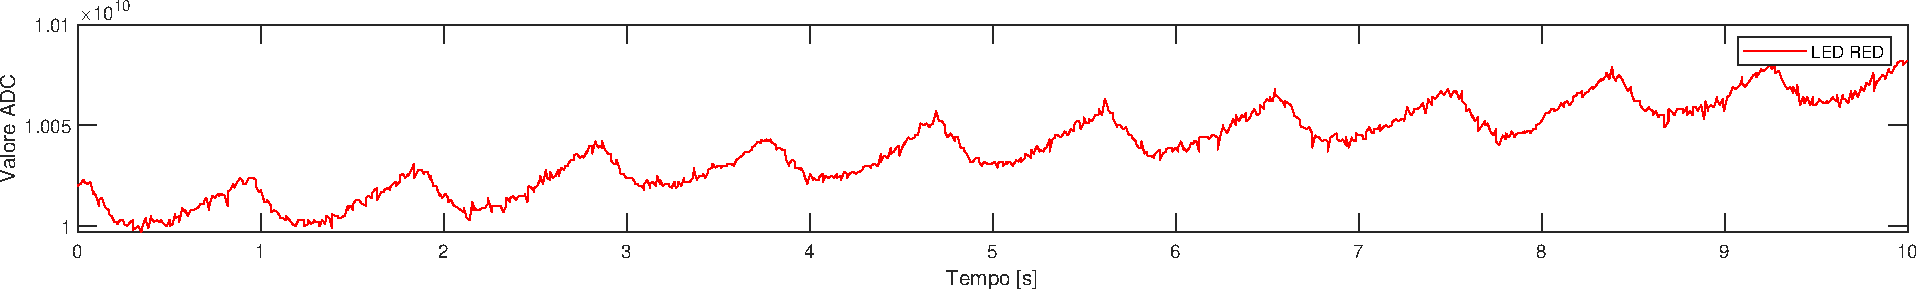
\includegraphics[width=1\linewidth]{ImageFiles/Misure Preliminari/Soggetto 2/max86916/polso_inferiore_red}
	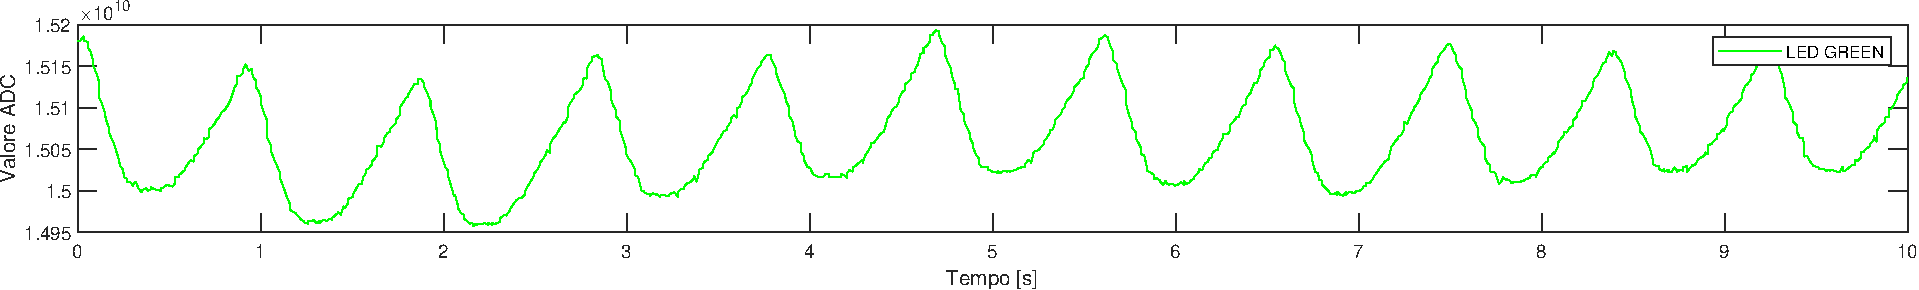
\includegraphics[width=1\linewidth]{ImageFiles/Misure Preliminari/Soggetto 2/max86916/polso_inferiore_green}
	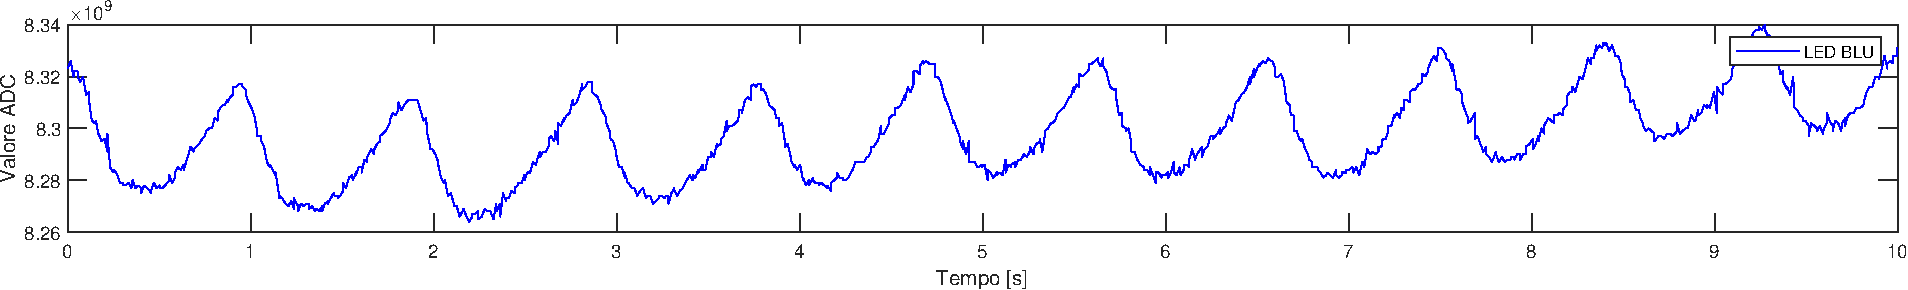
\includegraphics[width=1\linewidth]{ImageFiles/Misure Preliminari/Soggetto 2/max86916/polso_inferiore_blu}
	\caption{Segnali PPG acquisiti sul polso destro.}
	\label{fig:soggetto2_MAX86916_polso}
\end{figure}

\clearpage

\subparagraph{Fronte}

\begin{figure}[h]
	\centering
	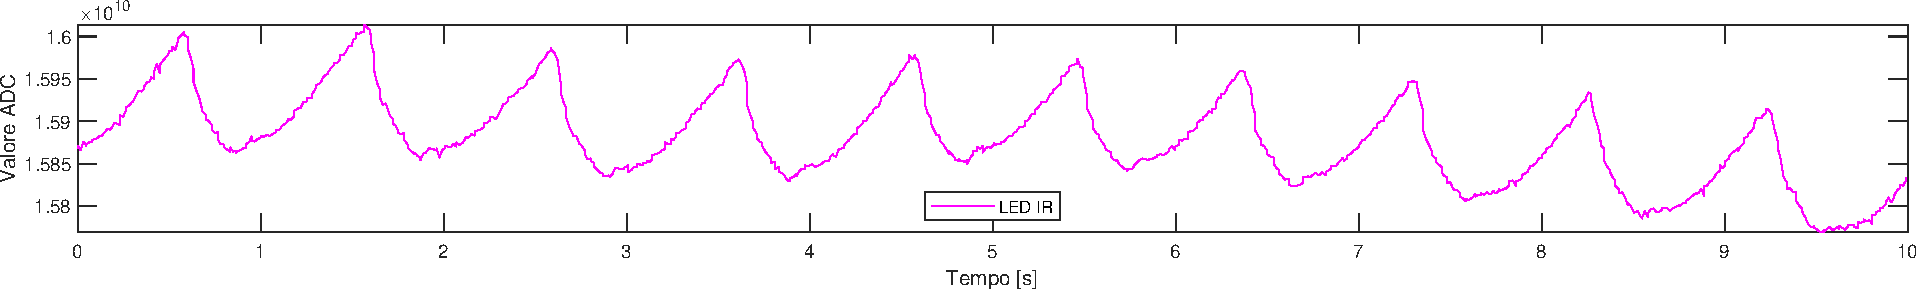
\includegraphics[width=1\linewidth]{ImageFiles/Misure Preliminari/Soggetto 2/max86916/fronte_ired}
	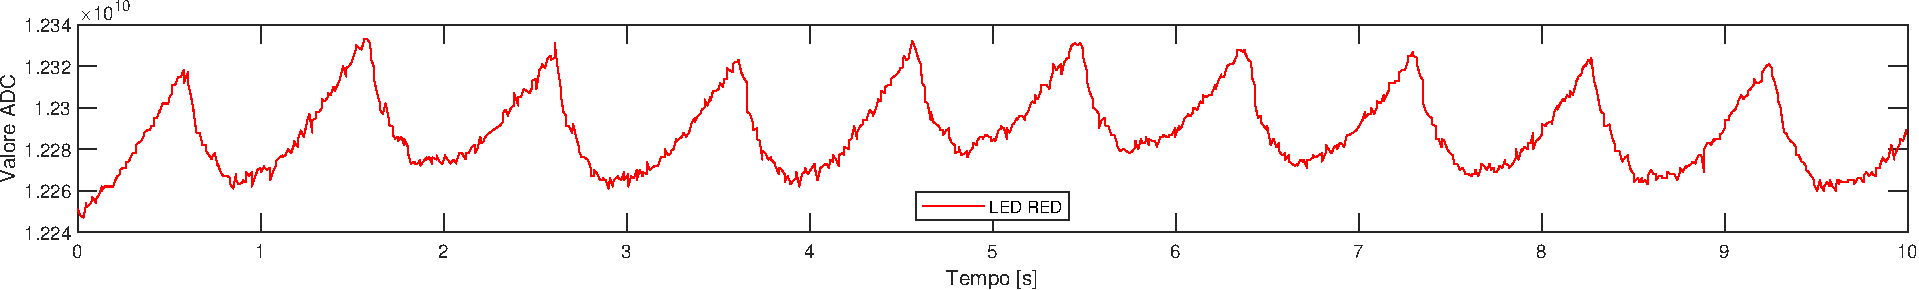
\includegraphics[width=1\linewidth]{ImageFiles/Misure Preliminari/Soggetto 2/max86916/fronte_red}
	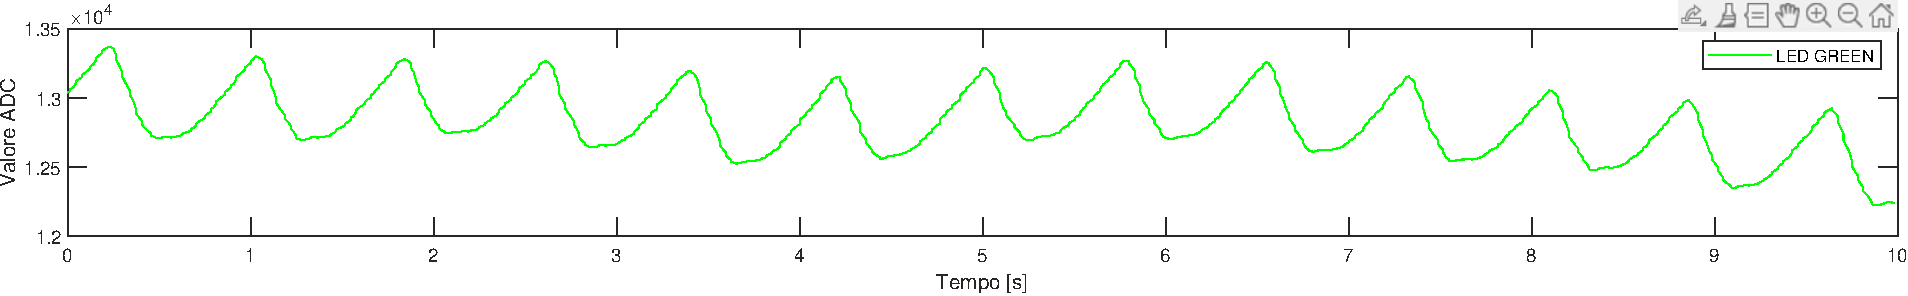
\includegraphics[width=1\linewidth]{ImageFiles/Misure Preliminari/Soggetto 2/max86916/fronte_green}
	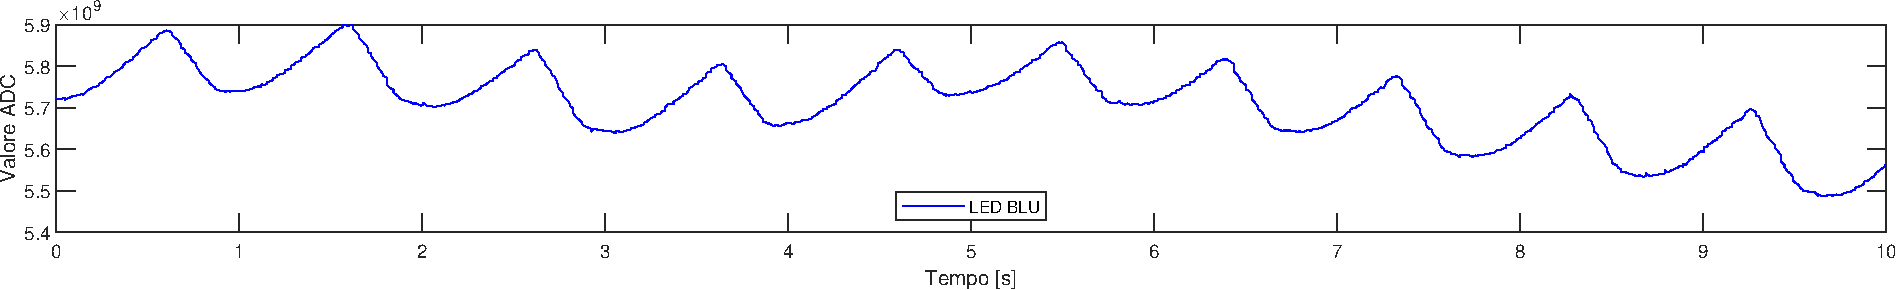
\includegraphics[width=1\linewidth]{ImageFiles/Misure Preliminari/Soggetto 2/max86916/fronte_blu}
	\caption{Segnali PPG acquisiti sulla fronte.}
	\label{fig:soggetto2_MAX86916_fronte}
\end{figure}






\clearpage